\documentclass[12pt]{article}

\usepackage[a4paper,margin=1in]{geometry}
\usepackage{amsmath,amssymb}
\usepackage{array}
\usepackage{booktabs}
\usepackage{enumitem}
\usepackage{graphicx}
\usepackage{hyperref}
\usepackage{xcolor}

\hypersetup{
  colorlinks=true,
  linkcolor=black,
  citecolor=blue!50!black,
  urlcolor=blue!50!black
}

\newcolumntype{L}[1]{>{\raggedright\arraybackslash}p{#1}}
\setlength{\emergencystretch}{2em}
\setcounter{tocdepth}{2}

\title{\textbf{Stability-Suppressed Leakage and Cross-Readout Residual Coherence}\\
\large A Synthetic Weak-Signal Amplification Protocol for Tau Core}
\author{Tau Core Research}
\date{Paper 16 draft package, 2026\\Last revised: 2026-08-26}

\begin{document}
\maketitle

\begin{abstract}
Tau Core is a readout-based research program in which observed physical
descriptions are treated as stabilized sector readouts of a deeper parent
morphological body.  A central methodological difficulty follows immediately:
if the observed world is a stable readout attractor, any direct leakage from the
parent layer into a single empirical sector should be small.  A decisive signal
may therefore not appear as one large anomaly in one channel, but as weak,
kernel-specific coherence across several heterogeneous residual channels.

This paper develops a synthetic methodology called the Weak-Signal
Amplification Protocol (WSAP).  WSAP tests whether several low-SNR readout
sectors can jointly recover a shared latent parent component better than any
single sector, while remaining specific against kernel-shuffle, common-noise,
phase-scramble, random-parent, and rotated-parent controls.  In the frozen
WSAP v1.0 hard-mode artifact studied here, all channels have target single
channel SNR about \(0.44\).  The best single-sector parent recovery is
\(0.361\), the joint parent recovery is \(0.673\), and the joint gain is
\(0.312\).  The specificity score is \(0.646\), while the main negative
controls remain near zero or anti-correlated with the true parent.

These numerical quantities are synthetic audit statistics.  They are not
p-values, likelihood ratios, physical detections, or validation-grade evidence
for Tau Core.  The paper's narrow claim is methodological: in a controlled
synthetic setting, weak heterogeneous residual readouts can recover a shared
latent parent more effectively in combination than individually, provided that
the protocol is forward-generative, held-out, and control-specific.
Because the channels are generated from a common synthetic parent, the result is
not surprising as a physical discovery.  The nontrivial part is the audit
structure: the parent is deliberately hidden behind lossy weak channels, no
single channel is allowed to dominate, and wrong-kernel/common-mode controls
must fail under the same scoring grammar.
\end{abstract}

\tableofcontents

\section{Scope and claim boundary}

This manuscript should be evaluated as a synthetic methodology and
claim-boundary paper, not as a phenomenological or empirical result paper.  It
does not analyze real astronomical data and does not claim physical validation
of Tau Core.

\noindent\textbf{Status:} Synthetic methodological demonstration only.

The main claim is deliberately narrow:
\begin{quote}
A shared weak parent component can be recovered from multiple heterogeneous,
low-SNR synthetic readouts better than from any single readout, provided the
recovery is forward-generative, held-out predictive, and specific against
negative controls.
\end{quote}

The paper does not claim that Tau Core is physically proven, that dark matter
or dark energy is explained, that lensing or galaxy rotation anomalies are
explained, that any real survey residual has been analyzed, or that the
synthetic parent used below is a realistic structure of nature.  The result is
a proof of method, not proof of world.

This distinction matters.  Without such a boundary, a positive synthetic result
could be misread as evidence for a new physical law.  Here it is used only to
sharpen a protocol: if future Tau Core real-data tests are attempted, they
should not search only for a single large residual in one sector.  They should
also test whether weak residuals in several sectors jointly preserve a
source-frozen parent signature.

Recovering a common latent component also does not identify the physical map
that transported it. In particular, terminal covariance cannot be inverted
into a smooth source arrow. Current Tau Core source accounting admits
non-scalar smooth transport only conditionally through full body-connection
holonomy or through Kato transport of a varying, constant-rank, source-owned
access projector. WSAP tests recoverability under a supplied synthetic map;
it neither selects nor physically occupies either transport mechanism.

The strongest criticism of any synthetic WSAP run is obvious and correct:
because the channels are generated from a shared parent, recovering shared
structure is not by itself remarkable.  The present package therefore treats the
shared-parent recovery as necessary but insufficient.  The synthetic task is
only meaningful if the parent is not trivially visible in any single sector, if
wrong readout kernels fail, if common structured noise does not masquerade as
the parent, and if held-out prediction remains positive.

\section{Position in the Tau Core program}

The current Tau Core picture can be summarized as
\[
  P_{\tau} \neq R_{3+1},
\]
where \(P_{\tau}\) denotes a parent morphological body and \(R_{3+1}\) denotes
the observed effective spacetime world.  The observed world is not treated as a
subjective illusion.  Rather, it is an effective readout:
\[
  R_{3+1} = \Pi_{B_{\rm phys}}(P_{\tau}).
\]
Observer-like systems are then internal to the readout,
\[
  O \subset R_{3+1},
\]
and may stabilize local compatible measurement states without creating the
global readout itself.

This paper uses only the methodological part of that picture.  It does not
derive \(P_{\tau}\), \(\Pi_{B_{\rm phys}}\), or a physical parent action.  It
asks a narrower question: if several readout sectors receive weak transformed
components from a shared parent, can a frozen protocol detect their joint
coherence while rejecting obvious controls?

\section{Stability-suppressed leakage}

The motivating Tau Core slogan is:
\begin{quote}
Stability suppresses amplitude; shared parent preserves coherence.
\end{quote}

If the effective \(3+1\)-dimensional readout is stable, then a large direct
parent leakage into one empirical sector would be suspicious.  The stability of
the observed sector suggests
\[
  \|\delta R_{\tau}\| \ll \|R_{3+1}\|.
\]
For a readout sector \(s\), write a residual in the schematic form
\[
  \epsilon_s = K_s \delta R_{\tau} + \eta_s + S_s,
  \label{eq:sector-residual}
\]
where \(K_s\) is the sector readout operator, \(\eta_s\) is random noise, and
\(S_s\) is structured systematic or selection contamination.

A single sector may therefore have
\[
  {\rm SNR}_s < 1.
\]
This is not by itself evidence for Tau Core.  It merely motivates the WSAP
question: after accounting for different sector kernels \(K_s\), does a common
latent component survive across sectors?

The target is not raw equality of residual maps,
\[
  \epsilon_L \approx \epsilon_R,
\]
which would be too naive.  The safer target is transformed coherence,
\[
  T_{L\to R}\epsilon_L \approx \epsilon_R,
  \qquad
  T_{L\to R}=K_R K_L^{-1},
\]
or, in practice, a joint forward fit in a compressed parent basis.

\section{Readout boundary and observer stabilization}

The package also records an observer/readout boundary intuition.  A local
observer-like system may be represented as
\[
  O_{\tau}=(I_O,B_O,E_O),
\]
with a Markov-blanket-like conditional structure
\[
  I_O \perp E_O \mid B_O.
\]
This is a structural analogy to conditional-independence boundaries and active
inference language \cite{Friston2010,Pearl2009}; it is not used as a physical
proof.  The local observer readout can be written
\[
  R_O=\Pi_{B_O}(R_{3+1})
      =\Pi_{B_O}\left(\Pi_{B_{\rm phys}}(P_{\tau})\right).
\]
The important point for WSAP is that different sector boundaries can yield
different readout operators:
\[
  R_s=\Pi_{B_s}(P_{\tau}).
\]
Thus cross-sector coherence cannot be tested by direct residual comparison
alone.  It must be tested through sector-aware kernels.

\section{WSAP as a finite protocol}

WSAP asks:
\begin{quote}
Can several weak heterogeneous residuals jointly reconstruct a shared latent
parent better than any single residual and better than negative controls?
\end{quote}

An idealized inverse problem is
\[
  \widehat P_{\tau}
  =
  \arg\min_P
  \left[
    \sum_s \|K_s(P)-\epsilon_s\|^2+\lambda C(P)
  \right],
  \label{eq:wsap-inverse}
\]
where \(C(P)\) is a complexity or morphology penalty and \(\lambda\) is a
regularization weight \cite{Tikhonov1963,Bishop2006}.  The synthetic
implementation uses a compressed parent basis,
\[
  P(c)=\sum_i c_iB_i,
\]
and solves a ridge-regularized forward fit in stacked readout space.

\subsection{What would make the synthetic test trivial?}

A synthetic parent experiment would be uninformative if any of the following
were true:
\begin{enumerate}[leftmargin=1.4em]
\item one channel directly encoded the parent map with high correlation;
\item the joint score remained high after assigning sectors to wrong kernels;
\item a smooth common-noise field produced the same apparent parent recovery;
\item phase-scrambled or rotated parents scored comparably to the true parent;
\item the reconstruction succeeded only on the training side and failed
held-out prediction.
\end{enumerate}
The v1.0 hard-mode criteria below are designed to block exactly these trivial
success modes.  They do not prove physical relevance; they only make the
synthetic method non-vacuous.

Figure~\ref{fig:protocol} shows the protocol structure.

\begin{figure}[t]
  \centering
  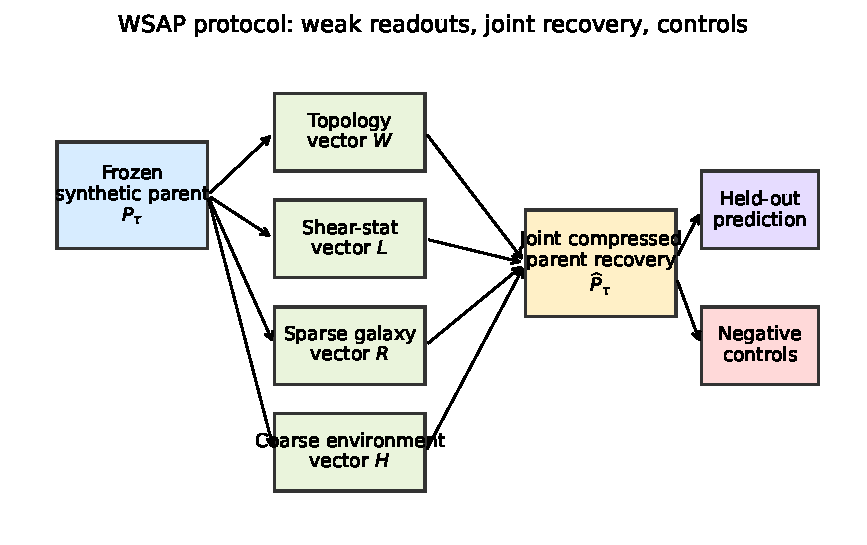
\includegraphics[width=0.95\linewidth]{figures/fig_wsap_protocol.pdf}
  \caption{WSAP protocol.  A frozen synthetic parent is passed through
  heterogeneous lossy readout channels.  The joint model attempts to recover a
  compressed parent representation and must survive held-out prediction and
  negative controls.}
  \label{fig:protocol}
\end{figure}

\section{Synthetic sectors}

The final v1.0 protocol uses four sectors.  These sectors are deliberately
synthetic analogues.  They are not survey products and should not be read as
actual cosmic-web, lensing, rotation, or Hubble analyses.

\subsection{\(W\): topology/statistics vector}

Earlier WSAP runs used \(W\) too close to a morphology map.  That made the
single-sector channel overly informative.  In v1.0, \(W\) is a topology and
statistics vector.  It includes threshold occupancy, gradient-weighted
occupancy, curvature summaries, anisotropy summaries, and block moments.  The
goal is to preserve weak structural information while suppressing direct
spatial reconstruction.

\subsection{\(L\): shear-statistics vector}

The \(L\) channel is a lensing-like shear-statistics vector.  Earlier runs used
too much map-like information.  In v1.0, \(L\) uses percentile summaries,
gradient percentiles, coarse strip summaries, and orientation-sensitive but
lossy information.  It is meant to be informative only in combination with
other sectors.

\subsection{\(R\): sparse galaxy-vector channel}

The \(R\) channel is sparse and point-sampled.  It uses galaxy-like sample
positions and vector residuals of the schematic form
\[
  R_i \sim
  aP(x_i)+b|\nabla P(x_i)|+c|\Delta P(x_i)|
  +{\rm contamination}.
\]
The point is not to model galaxy rotation curves.  The point is to test a
readout whose sampling is sparse and local.

\subsection{\(H\): coarse environment channel}

The \(H\) channel is a coarse environment-like readout.  It uses smoothed
parent information and lossy binning into void/intermediate/node-like regions.
It is intentionally coarse, because a strong environment map would make the
synthetic task too easy.

\section{Implementation and reproducibility grade}

The current repository is a reproducible paper package for the frozen WSAP v1.0
result artifact.  It recomputes headline summary metrics from the frozen JSON
artifact, rebuilds figures, compiles the paper, builds an arXiv source package,
and runs smoke tests.  It is not yet a full raw-run replay package from the
original random-number seed and feature matrices.

For audit clarity, Table~\ref{tab:implementation-ledger} separates what is
currently fixed from what a stronger v1.1 package should expose.

\begin{table}[t]
\centering
\small
\begin{tabular}{L{0.26\linewidth}L{0.32\linewidth}L{0.30\linewidth}}
\toprule
Item & Current v1.0 package & Required for audit-grade v1.1\\
\midrule
Parent generator & Frozen result artifact records the recovered metrics &
Raw parent generator, random seed, grid size, basis functions\\
Feature extraction & Channel classes are described; final features are
summarized by sector & Exact feature dimensions, masks, normalizations, and
transform matrices\\
Noise model & Target SNR and control outcomes are frozen & Explicit noise
distribution, covariance model, and contamination amplitudes\\
Fit rule & Ridge-regularized stacked forward fit is declared & Exact design
matrix, ridge parameter, centering/scaling, and solver tolerance\\
Held-out rule & Held-out correlations are frozen & Exact train/held-out split,
split seed, and replay script from raw features\\
Thresholds & Thresholds and margins are reported & Predeclared threshold file
plus sensitivity sweep across nearby thresholds\\
Stress grid & Not part of the v1.0 result artifact & Sweep thresholds, ridge
\(\lambda\), SNR, feature dimensions, and held-out split stability\\
Mock injection & Not included & Realistic mock-catalog injection with known
parent and control components\\
Independent replay & Not included & Separate implementation from the frozen
protocol, not shared analysis code\\
\bottomrule
\end{tabular}
\caption{Implementation ledger.  The current package is result-artifact
reproducible, not yet raw-generator reproducible.  This is acceptable for a
methodology note but must be upgraded before any stronger claim.}
\label{tab:implementation-ledger}
\end{table}

\section{Pass/fail criteria}

The v1.0 synthetic hard-mode criteria are:
\[
  \max_s {\rm corr}(\widehat P_s,P_{\tau}) < 0.75,
  \label{eq:single-suppression}
\]
so no single sector may reconstruct the parent too well;
\[
  {\rm corr}(\widehat P_{\rm joint},P_{\tau})
  -
  \max_s {\rm corr}(\widehat P_s,P_{\tau})
  >0.10,
  \label{eq:joint-gain}
\]
so the joint model must improve on the best single sector;
\[
  \overline{{\rm corr}}_{\rm heldout,noisy}>0.18,
  \label{eq:heldout}
\]
so held-out prediction must be positive; and
\[
  S_{\rm specificity}>0.30,
  \label{eq:specificity-threshold}
\]
so the candidate must survive negative controls.

These thresholds are protocol thresholds for the synthetic audit.  They are not
universal constants and must be redefined for any future mock-catalog or real
data application.

The threshold choices are guardrails rather than fitted constants.  The
single-sector bound \(0.75\) rejects cases where one channel already exposes the
parent too directly.  The joint-gain bound \(0.10\) requires a visible
multi-channel advantage over the best single sector.  The held-out bound
\(0.18\) requires positive out-of-sample behavior above a weak-noise floor.  The
specificity bound \(0.30\) requires substantial separation from the principal
controls.  Table~\ref{tab:threshold-margins} reports the margins in the frozen
v1.0 artifact.

\begin{table}[t]
\centering
\small
\begin{tabular}{L{0.33\linewidth}rrr}
\toprule
Criterion & Threshold & v1.0 value & Margin\\
\midrule
Best single-sector recovery & \(<0.75\) & 0.3606 & 0.3894 below cap\\
Joint gain over best single & \(>0.10\) & 0.3123 & 0.2123 above floor\\
Mean held-out noisy prediction & \(>0.18\) & 0.4110 & 0.2310 above floor\\
Specificity score & \(>0.30\) & 0.6464 & 0.3464 above floor\\
\bottomrule
\end{tabular}
\caption{Threshold rationale and v1.0 margins.  These are not universal Tau
Core constants; they are synthetic audit guardrails.}
\label{tab:threshold-margins}
\end{table}

\section{Negative controls}

A WSAP candidate is not meaningful unless it fails the obvious ways in which a
multi-channel method can fool itself.

\begin{description}[leftmargin=2.4cm,style=nextline]
\item[Kernel shuffle.]
Sector targets are assigned to wrong readout operators.  If recovery remains
strong, the result is not sector-specific.
\item[Common-mode structured noise.]
A smooth nuisance field is passed through comparable targets.  If the Tau
component recovers the true parent under common noise, the method is
overfitting.
\item[Phase scramble.]
The parent spectral amplitude is kept while phase is randomized.  If recovery
remains strong, morphology is not specific.
\item[Random parent.]
A random smooth field tests accidental correlation.
\item[Rotated parent.]
The parent is spatially rotated to test loose morphology matching.
\end{description}

The specificity score used in the package is
\[
  S_{\rm specificity}
  =
  S_{\rm real}
  -
  S_{\rm shuffle}
  -
  S_{\rm common}
  -
  \frac12|S_{\rm phase}|.
  \label{eq:specificity}
\]
In implementation form,
\[
\begin{aligned}
S_{\rm specificity}
&=
{\rm corr}(\widehat P_{\tau},P_{\tau})
-\max(0,{\rm corr}(P_{\rm shuffle},P_{\tau}))\\
&\quad
-\max(0,{\rm corr}(P_{\rm common},P_{\tau}))
-\frac12
\left|{\rm corr}(P_{\rm phase},\widehat P_{\tau})\right|.
\end{aligned}
\]

\section{Frozen v1.0 synthetic result}

All channels in the final artifact have target single-channel SNR about
\[
  {\rm SNR}_s=0.44.
\]
The single-sector recoveries are listed in Table~\ref{tab:single}.  The best
single sector is \(H\), with parent recovery \(0.3606\).

\begin{table}[t]
\centering
\begin{tabular}{L{0.52\linewidth}r}
\toprule
Sector & Parent recovery\\
\midrule
\(W\) / topology vector & 0.0488\\
\(L\) / shear-stat vector & -0.0242\\
\(R\) / sparse vector & 0.3192\\
\(H\) / coarse environment & 0.3606\\
\bottomrule
\end{tabular}
\caption{Single-sector parent recovery in the frozen WSAP v1.0 synthetic
artifact.}
\label{tab:single}
\end{table}

The joint parent recovery is
\[
  {\rm corr}(\widehat P_{\rm joint},P_{\tau})=0.6729,
\]
and the joint gain is
\[
  0.6729-0.3606=0.3123.
\]
This satisfies the synthetic criterion in Eq.~\eqref{eq:joint-gain}.

\begin{figure}[t]
  \centering
  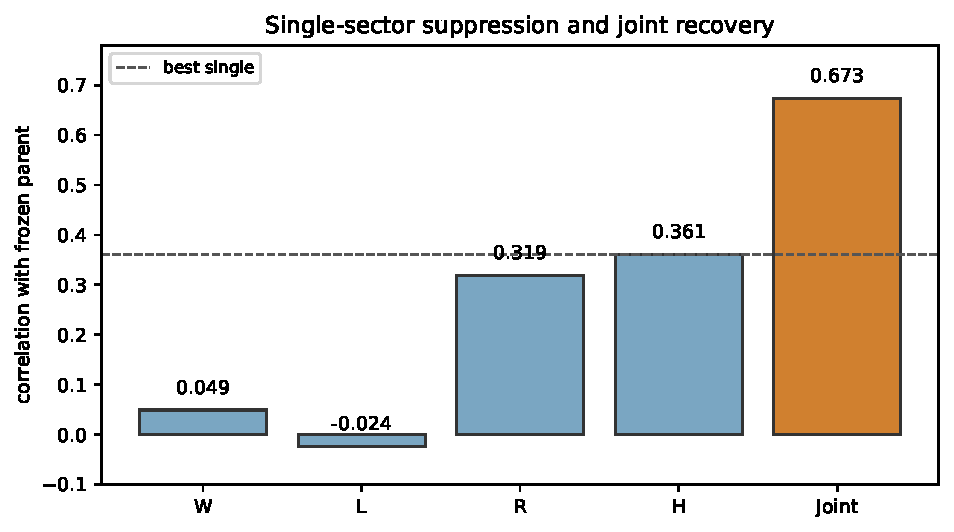
\includegraphics[width=0.88\linewidth]{figures/fig_single_vs_joint.pdf}
  \caption{Single-sector suppression and joint recovery.  The joint synthetic
  model recovers the frozen parent more strongly than any single channel.}
  \label{fig:single-joint}
\end{figure}

\section{Held-out behavior}

Held-out prediction is important because a joint reconstruction can look
strong on the training side while failing to generalize.  Table~\ref{tab:heldout}
reports the frozen held-out correlations.

\begin{table}[t]
\centering
\begin{tabular}{lrrr}
\toprule
Sector & Parent from training & Noisy residual & Hidden signal\\
\midrule
\(W\) & 0.6563 & 0.6391 & 0.9238\\
\(L\) & 0.6829 & 0.5143 & 0.8840\\
\(R\) & 0.3196 & 0.2622 & 0.6837\\
\(H\) & 0.5514 & 0.2284 & 0.5532\\
\bottomrule
\end{tabular}
\caption{Held-out synthetic prediction.  The noisy-residual column is the
conservative held-out score; the hidden-signal column is available only because
this is a synthetic audit.}
\label{tab:heldout}
\end{table}

The mean held-out noisy prediction is
\[
  \overline{{\rm corr}}_{\rm heldout,noisy}=0.4110,
\]
and the mean hidden-signal prediction is
\[
  \overline{{\rm corr}}_{\rm heldout,hidden}=0.7612.
\]
Only the noisy held-out score would be available in an endpoint-like real-data
setting.  The hidden score is a synthetic diagnostic.

\begin{figure}[t]
  \centering
  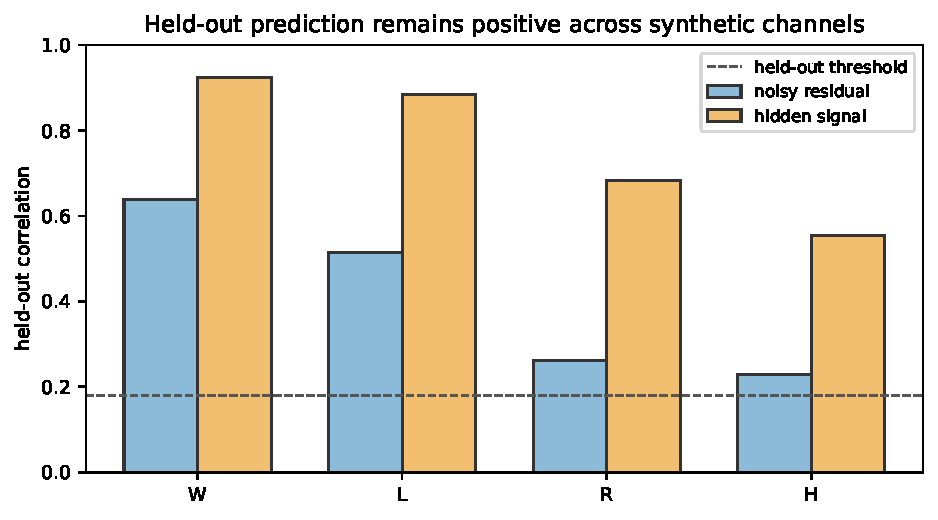
\includegraphics[width=0.88\linewidth]{figures/fig_heldout_prediction.pdf}
  \caption{Held-out prediction remains positive across synthetic channels.
  The hidden signal bars are diagnostic only; real data would not provide them.}
  \label{fig:heldout}
\end{figure}

\section{Control separation}

The main controls are summarized in Table~\ref{tab:controls}.  The controls are
not all expected to be negative in every auxiliary diagnostic.  The primary
criterion is that the Tau-parent recovery and specificity score separate the
candidate from wrong-kernel and non-specific alternatives.

\begin{table}[t]
\centering
\begin{tabular}{L{0.62\linewidth}r}
\toprule
Control & Result\\
\midrule
Kernel-shuffle Tau parent correlation & -0.0507\\
Common-noise Tau correlation with true parent & -0.3892\\
Phase-scrambled correlation with joint Tau & -0.0531\\
Random-parent correlation with joint Tau & 0.0940\\
Rotated-parent correlation with joint Tau & 0.0789\\
\bottomrule
\end{tabular}
\caption{Primary negative controls.  Controls remain far below the joint
candidate correlation \(0.6729\).}
\label{tab:controls}
\end{table}

The specificity score is
\[
  S_{\rm specificity}=0.6464,
\]
which satisfies Eq.~\eqref{eq:specificity-threshold}.

\begin{figure}[t]
  \centering
  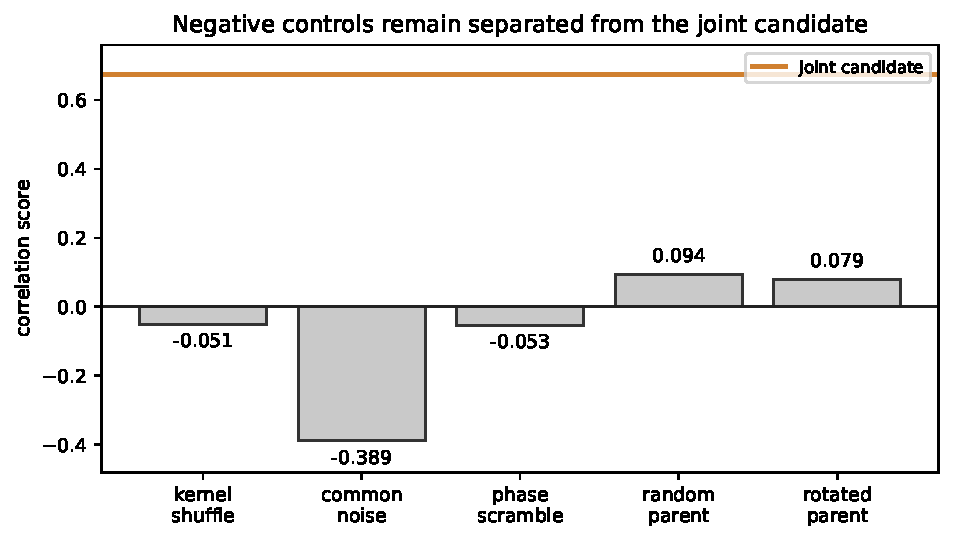
\includegraphics[width=0.88\linewidth]{figures/fig_negative_controls.pdf}
  \caption{Control separation.  Signed control values near zero or negative
  indicate that wrong-kernel or non-specific alternatives do not recover the
  frozen parent under the same statistic.}
  \label{fig:controls}
\end{figure}

\section{Development history}

The v1.0 result was not the first attempt.  The development history is
important because it preserves negative and partial results.  Earlier runs
failed or only partially passed because individual channels were too visible,
kernel shuffling was too permissive, or common-mode structure leaked into the
Tau component.  This is not a nuisance detail: it is the main reason the v1.0
claim is methodological rather than rhetorical.

The development history should be read as exploratory until v1.0.  Versions
v0.1--v0.9 are preserved because they document how trivial success modes were
found and blocked.  They are not independent confirmation.  The frozen v1.0
artifact is the first package-level confirmatory target within this synthetic
line, and even that target remains internal to the synthetic family.  A
stronger paper would need a v1.1 raw-generator replay, sensitivity sweep,
mock-catalog injection test, and independent reimplementation.

\begin{figure}[t]
  \centering
  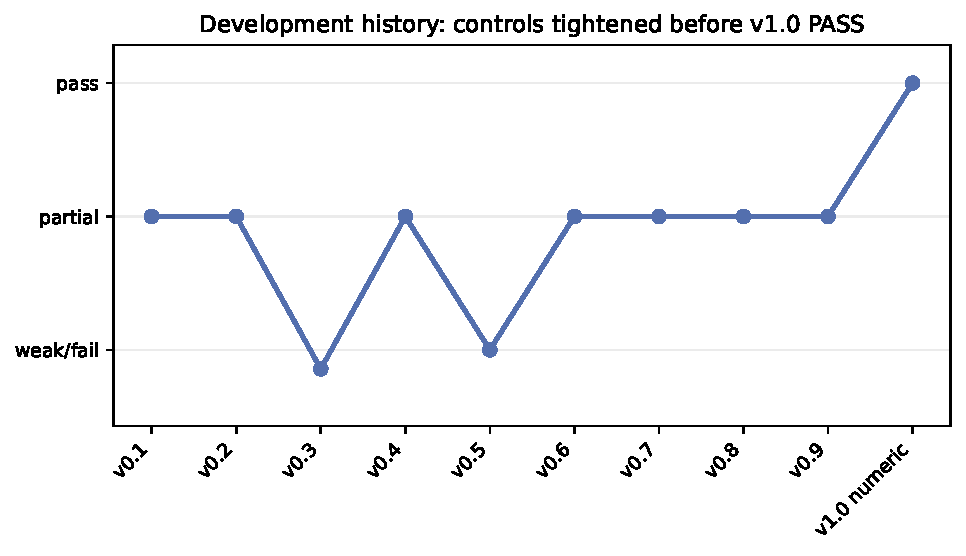
\includegraphics[width=0.90\linewidth]{figures/fig_development_history.pdf}
  \caption{Development history from v0.1 to v1.0.  The final PASS follows
  progressive tightening of controls and lossy vectorization of overly
  informative channels.}
  \label{fig:history}
\end{figure}

\begin{table}[t]
\centering
\small
\begin{tabular}{L{0.17\linewidth}L{0.20\linewidth}L{0.50\linewidth}}
\toprule
Version & Verdict & Key lesson\\
\midrule
v0.1 & Partial pass & Weak signals combined, but shuffle too permissive.\\
v0.3 & Weak/fail & Backprojection averaging was insufficient.\\
v0.5 & Weak/fail & Common-mode structure could still leak into Tau.\\
v0.8 & Partial pass & \(W\) vectorization helped but joint gain too small.\\
v0.9 & Partial pass & Controls good, but \(L\) remained too informative.\\
v1.0 & Pass & \(W,L\) vectorized; \(R\) sparse; \(H\) coarse; joint gain passed.\\
\bottomrule
\end{tabular}
\caption{Compressed development ledger.  The full version history is included
in `data/derived/version\_history.csv'.}
\label{tab:history}
\end{table}

\section{Why this matters for Tau Core}

The result supports a methodological expectation, not a physical conclusion.
Tau Core should not necessarily expect one large anomaly in one sector.  A
more characteristic pattern may be
\[
  {\rm weak\ single\ sector\ residuals}
  +
  {\rm cross\ readout\ coherence}.
\]
This paper shows that such a pattern can be recovered in principle in a
controlled synthetic setting.

The result is also compatible with the broader residual cross-readout support
discipline developed elsewhere in the Tau Core program: a candidate residual
becomes more interesting when independent readout sectors preserve a shared
source-frozen signature, and less interesting when the effect is dominated by
one channel, a wrong kernel, or common-mode noise.

The foundation-level common-ancestor result sharpens this interpretation.  If
the weak channels are physical descendants of one descriptor \(\Xi_{OS}\),
then every admitted channel must be constant on its fibres; the joint stack
recovers the full local descriptor only when its Jacobian kernel equals
\(\ker D\Xi_{OS}\).  WSAP assumes a shared latent source in its synthetic
generator but does not prove either physical factorization or this kernel
equality.  Its positive result is therefore a method witness, not a
common-ancestor theorem.

\section{Relation to earlier Tau Core readout papers}

The role of this paper is different from the galaxy and cosmology endpoint
papers in the Tau Core sequence.  Earlier work asked whether particular
readout families, morphology labels, observer/path kernels, or cosmological
channels could be frozen source-side and then replayed against endpoint-like
statistics.  Those papers are closer to prevalidation or empirical protocol
work.  Paper 16 instead asks a meta-methodological question: if each individual
readout is weak, can a source-frozen joint protocol still recover a shared
parent component under synthetic control?

This distinction prevents a common overclaim.  A positive WSAP result does not
mean that galaxy kernels, cosmological kernels, or lensing/path kernels are
physically correct.  It means that the cross-readout strategy is not obviously
empty as a signal-processing architecture.  It shows that weak residual
channels can, in principle, be designed so that the correct joint kernel
outperforms single-sector and wrong-kernel alternatives.

Paper 17 adds a stricter downstream classifier for this situation.  It reports
shared-parent covariance support \(Z_{\rm shared}\) separately from
morphology/orientation support \(Z_{\rm orient}\).  In that classifier,
orientation-only structure is a control or warning class rather than evidence
by itself.  A future WSAP endpoint should therefore avoid counting visually
aligned or morphology-like residual structure as parent recovery unless the
shared-parent covariance axis also survives.

\begin{table}[t]
\centering
\small
\begin{tabular}{L{0.23\linewidth}L{0.32\linewidth}L{0.32\linewidth}}
\toprule
Tau Core direction & What those papers test & What WSAP adds\\
\midrule
Morphology-forward galaxy readouts & Whether source-frozen morphology
families improve rotation residual structure & A generic weak-channel
combination grammar\\
Observer/path projection readouts & Whether observer/path information changes
the selected kernel & A control language for multi-channel coherence rather
than single-kernel improvement\\
Cosmology readouts & Whether void, web, path, and time-like channels
survive source-side audits & A synthetic demonstration of joint weak-channel
recovery\\
Foundation/readout language & How to state parent/readout/null/relift objects
without overclaiming & A concrete finite protocol using that language\\
\bottomrule
\end{tabular}
\caption{Paper 16 is not a replacement for endpoint papers.  It is a
methodological bridge explaining why multi-readout weak-signal tests are worth
constructing.}
\label{tab:sequence}
\end{table}

\section{Operational freeze ledger}

The most important real-data lesson from WSAP is not the synthetic PASS.  It is
the need for a strict freeze ledger before endpoint scoring.  A serious future
WSAP test must define, before looking at endpoint residual success, all of the
following:

\begin{table}[t]
\centering
\small
\begin{tabular}{L{0.24\linewidth}L{0.34\linewidth}L{0.30\linewidth}}
\toprule
Ledger item & What must be frozen & Why it matters\\
\midrule
Sector list & Which readout sectors enter the joint statistic & Prevents
adding sectors after seeing a favorable residual\\
Feature extraction & Maps, vectors, summaries, smoothing, masks, and
normalizations & Prevents endpoint leakage through preprocessing\\
Parent basis & Basis functions or latent parameterization & Prevents
over-flexible parent reconstruction\\
Regularization & Ridge weight, complexity penalty, or prior & Prevents
amplitude rescue after the fact\\
Negative controls & Shuffle, common-mode, phase, random, rotated, and
survey-specific controls & Defines what counts as non-specific success\\
Held-out split & Training/holdout or block split rule & Prevents scoring on
the same structure used to build the kernel\\
Pass/fail thresholds & Numerical criteria and failure states & Prevents
retroactive reinterpretation\\
\bottomrule
\end{tabular}
\caption{Minimum freeze ledger for a future non-synthetic WSAP protocol.}
\label{tab:freeze-ledger}
\end{table}

This ledger is intentionally stricter than an exploratory analysis.  The point
is not to maximize the apparent Tau Core signal.  The point is to create a
protocol that can fail cleanly.

\section{Real-data roadmap}

A real-data WSAP program would require much more than the present paper.
The roadmap is:

\begin{enumerate}[leftmargin=1.4em]
\item Build a v1.1 raw-generator replay: random seed, parent generator, feature
matrix, noise model, covariance rule, train/held-out split, ridge
\(\lambda\), and solver tolerance must regenerate the result from raw
synthetic ingredients.
\item Freeze the protocol before endpoint scoring: sector definitions, feature
extraction, thresholds, controls, and held-out scheme.
\item Run sensitivity sweeps over thresholds, ridge \(\lambda\), SNR,
feature dimensions, and held-out split stability without selecting the best
score after the fact.
\item Run mock-catalog injection with realistic covariance, masks, and
selection effects.
\item Use semi-real public simulations to test whether injected parent-like
signals can be separated from baryonic, environmental, and survey systematics.
\item Require an independent implementation that rebuilds the protocol from the
frozen specification.
\item Only then attempt a blind real-data pilot.
\item Require independent replication on a second dataset or survey region.
\end{enumerate}

Candidate future sectors include weak-lensing residual statistics
\cite{KiDS1000}, SPARC-like rotation residual summaries \cite{SPARC},
cosmic-web topology descriptors, and supernova or expansion residuals by
environment.  This list is a roadmap, not a claim that these data already
support Tau Core.

\section{Falsification and failure criteria}

The WSAP branch weakens if any of the following patterns appear:

\begin{enumerate}[leftmargin=1.4em]
\item recovery is always driven by one sector;
\item joint gain disappears under realistic covariance;
\item specificity is zero or negative;
\item common-mode structured noise performs as well as the Tau candidate;
\item kernel shuffle performs as well as correct operators;
\item held-out prediction collapses;
\item results depend on arbitrary feature choices;
\item independent replication fails.
\end{enumerate}

For real data, a strong negative result would be a source-frozen, blinded,
multi-sector protocol in which the matched kernels fail while shuffled,
common-mode, or wrong-parent controls perform equally well or better.  Such a
result should be preserved, not tuned away.

\section{Reproducibility package}

The repository provides a one-command reproduction path:
\[
  \texttt{python scripts/reproduce.py}.
\]
The command regenerates the synthetic summary table, builds the figures,
compiles the PDF, builds the arXiv source zip, and runs smoke tests.  The
tests verify that the frozen numbers are present, that claim-boundary markers
are included, and that the arXiv zip is source-only.

The frozen synthetic metrics are stored in
\[
  \texttt{data/derived/results\_v10\_numeric.json}.
\]
The recomputed pass/fail summary is written to
\[
  \texttt{data/derived/wsap\_v10\_recomputed\_summary.csv}.
\]

\section{Artifact ledger}

The compact reproducibility package contains the following core artifacts:

\begin{center}
\small
\begin{tabular}{L{0.36\linewidth}L{0.49\linewidth}}
\toprule
Artifact & Role\\
\midrule
\texttt{data/derived/}\newline\texttt{results\_v10\_numeric.json} & Frozen numerical result
artifact from the WSAP v1.0 synthetic package\\
\texttt{data/derived/}\newline\texttt{v10\_results\_table.csv} & Flat table of headline
metrics, controls, and held-out values\\
\texttt{data/derived/}\newline\texttt{version\_history.csv} & Preserved development history,
including partial and weak/fail stages\\
\texttt{scripts/}\newline\texttt{run\_wsap\_synthetic.py} & Recomputes summary metrics and
pass/fail flags from the frozen artifact\\
\texttt{scripts/}\newline\texttt{build\_figures.py} & Regenerates all paper figures from
frozen artifacts\\
\texttt{scripts/}\newline\texttt{reproduce.py} & One-command reproduction path\\
\texttt{tests/}\newline\texttt{test\_public\_}\newline\texttt{reproducibility\_package.py} & Smoke tests for
claim boundaries, frozen metrics, PDF existence, and arXiv source packaging\\
\bottomrule
\end{tabular}
\end{center}

The repository intentionally does not include private workbench logs or broad
exploration dumps.  Negative and partial results are preserved in the version
history, while the public package remains compact enough for independent
inspection.

\section{Relation to the full-4D fixed score}

The synthetic WSAP specificity score tests protocol recovery and wrong-family
separation.  It is not the later physical full-4D score.  That score requires
a source-frozen tensor
\[
 E_g={1\over\mathcal A_*}(A_O^{(4)-1})^*
 \left[(K_{HH}-K_{\rm std})-CK_{VV}^{-1}C^\dagger\right]
 A_O^{(4)-1}
\]
and the stacked prediction $\mu_\tau=\bigoplus_a\mathcal T_a[E_g]$, with exact
duplicates removed and genuine terminal overlap retained through the full
covariance.  The present synthetic package establishes neither physical
occupation nor a nonzero $E_g$; its reported specificity values therefore
remain synthetic diagnostics and are not recomputed.

% BEGIN OBSERVER UPDATE 20260914
\section{Observer realization: inherited results and physical boundary}
\label{sec:observer-update-20260914}
The current observer programme distinguishes a conditional mathematical
construction from an occupied physical measuring system. The source order
remains base plus one universal seed, stabilized morphological response,
observer--source restriction, shared descriptor, and resolved terminal
readouts. Neither a detector nor an empirical residual constructs the parent
body backwards. Dynamics below concern downstream subsystems only.

The canonical observer-origin derivation, Sections 22--26, owns the following
results. The existing joint source action fixes static and frequency-dependent
response together. Variation of the BRAC potential couples to the field
square; a linear field coupling is a distinct comparator unless derived by
expansion about an occupied background. Fixed canonical means select a unique
coherent state in a finite positive harmonic packet only if there is no excess
fluctuation energy. This is a free/asymptotic preparation statement, not the
ground state of an interacting detector. For the existing coupled harmonic
pair, the joint ground is pure but either local subsystem is mixed, with its
covariance fixed by the complete joint Hamiltonian.

These are conditional derivations and internal numerical checks. The actual
observer--source context, physical preparation process, kinetic/energy
calibration and stable operational resolution remain unproved. The existing
ORA-T1 selector conditionally chooses stable quantizers when the occupied
context, admissible partition family and positive closure barrier are supplied;
it does not establish those physical premises. A computed ground state is not
a preparation mechanism, and a covariance or optimal abstract measurement is
not an implemented stable quantizer $Q_{OS}$.

\paragraph{Ownership and use.}
The central observer-origin note owns the new contact, state and covariance
derivations; the body-readout technical companion carries the consolidated
mathematics. Foundation Papers IV, V and VI retain physical-selection,
clock-descent and quantum-readout ownership, respectively. This paper imports
only the consequences within its scope. No observational dataset, baseline,
frozen coefficient, score or empirical conclusion is revised by this update.
The reproducibility supplement records the source hashes and the exact
conditional/physical distinction.


\paragraph{Consequence for this paper.}
Different terminal labels are not independent information sources without a factorization or novelty proof. A nonzero correlation is not automatically a standard-orthogonal Tau signal.
% END OBSERVER UPDATE 20260914

% BEGIN STATE UPDATE 20260918
\section{Source identification and recovery}
The current observer audit separates a conditional forward construction from physical source selection. A frozen body, occupied observer incidence, preparation, complete instrument and stable resolution can determine records without selecting those inputs from Nature. Equal effects do not fix postmeasurement states, and symmetry within a chosen interaction family does not exclude other symmetric couplings. Different terminal labels are not independent information sources without a factorization or novelty proof. A nonzero correlation is not automatically a standard-orthogonal Tau signal.

\paragraph{Dependency and claim ownership.}
Foundation VI and the body--readout technical companion own the finite instrument/access proof; Foundation IV and TD-0 retain physical source selection; Foundation V, the temporal synthesis and seed--body companion own the gradient/inertial distinction. This paper inherits only the stated specialization. Canonical assumptions, countermodels and calibration audits are in \url{https://github.com/tau-core-research/tau-core-theory/blob/main/docs/tau_rqm_instrument_to_record_bridge_001.md}. No physical seed, Nature occupation or Tau-exclusive observation is established by this update. Existing empirical endpoint definitions and scores are unchanged.
% END STATE UPDATE 20260918

% BEGIN PAIR READOUT UPDATE 20260927
\section{Conditional source preparation and time-resolved access}
The common-operator scalar--Dirac completion now supports an explicit
conditional chain from interaction vertices to pair transfer and joint
readout. Nonzero vertices do not select occupation. Relational coherence
can be generated from an occupied number-diagonal pair even while both
local mean fields vanish. In a declared resonant rotating-wave and Markov
loss model, finite-window emission retains this coherence information,
whereas an all-time count discards it. This is standard-compatible quantum
recovery, not a Tau-specific observational residual.
Different terminal labels are not independent information sources without a factorization or novelty proof. A nonzero correlation is not automatically a standard-orthogonal Tau signal.
\paragraph{Dependency ownership and limits.}
The P4 common-source assembly owns the scalar/Yukawa benchmark and finite
preparation calculations; Foundation VI and the body--readout companion
inherit the joint-access mathematics. Foundation IV and TD-0 retain
physical source selection, and Foundation V retains clock descent.
The parent remains atemporal: the evolution above is a conditional
downstream 4D model, not parent memory or a derived morphogenetic time.
Physical initial occupation, a gauge-complete realization, detector
amplification, absolute calibration and stable observer-relative $Q_{OS}$
remain unselected. No empirical endpoint or score is changed.
The canonical derivation and reproducible numerical sources are linked at
\url{https://github.com/tau-core-research/tau-core-theory/blob/main/docs/tau_core_p4_nonabelian_particle_common_source_assembly_001.md}.
% END PAIR READOUT UPDATE 20260927

\section{Conclusion}

WSAP v1.0 is a synthetic hard-mode PASS.  In the frozen artifact, each sector
is weak, the best single-sector recovery is \(0.361\), the joint recovery is
\(0.673\), the joint gain is \(0.312\), held-out prediction remains positive,
and the specificity score is \(0.646\).  The principal controls remain
separated from the joint candidate.

The result should be read narrowly.  It does not validate Tau Core physically.
It demonstrates that the Tau Core weak-signal strategy is methodologically
coherent enough to deserve mock-catalog and eventually blind real-data testing.
The next scientific step is not to strengthen the claim, but to freeze a
realistic mock-catalog WSAP protocol and let it fail or pass under realistic
covariance, masks, systematics, and independent replication.

\bibliographystyle{plain}
\bibliography{refs}

\end{document}
